\documentclass[mathNotesPreamble]{subfiles}
\begin{document}
%\relscale{1.4}
\section{4.1: Maxima and Minima}
\begin{defn*}[Absolute Maximum and Minimum]
  Let $f$ be defined on a set $D$ containing $c$. 
  \begin{itemize}
    \item 
      If $f(c)\geq f(x)$ for every $x$ in $D$, then $f(c)$ is an \textbf{absolute maximum} value of $f$ on $D$.
    \item 
      If $f(c)\leq f(x)$ for every $x$ in $D$, then $f(c)$ is an \textbf{absolute minimum} value of $f$ on $D$.
    \item 
      An \textbf{absolute extreme value} is either an absolute maximum value or an absolute minimum value.
  \end{itemize}
\end{defn*}
\vspace*{\stretch{1}}
\begin{ex*}
  Determine whether the function has any absolute extreme values
\end{ex*}
\begin{center}
  \begin{tikzpicture}
    \begin{groupplot}[
      group style={group size=3 by 2, horizontal sep=2cm, vertical sep=2cm},
      axis lines=center,
      axis line style={->},
      width=0.3\linewidth,
      ticklabel style={font=\footnotesize,inner sep=0.5pt,fill=white,opacity=1.0, text opacity=1},
      xlabel=$x$, xlabel style={at={(ticklabel* cs:1)},anchor=north west},
      ylabel=$y$, ylabel style={at={(ticklabel* cs:1)},anchor=south},
      every axis plot/.append style={line width=0.95pt, color=blue}
      ]
      \nextgroupplot[
        xmin=-6, xmax=6,
        ymin=-6, ymax=6,
        ylabel=${y=-x^2+4}$, 
        ]
        \addplot[<->] expression[domain=-3:3]{-x^2+4};
      \nextgroupplot[
        xmin=-6, xmax=6,
        ymin=-6, ymax=6,
        ylabel=${y=\frac{x^3}{3}+x^2+1}$,
        ]
        \addplot[<->] expression[domain=-4.125:1.775]{x^3/3+x^2+1};
      \nextgroupplot[
        xmin=-6.75, xmax=6.75,
        ymin=-1.5, ymax=1.5,
        ylabel=${y=\sin(x)}$,
        xtick={-6.28318, -3.141592, ..., 6.28318},
        xticklabels={$-2\pi$,$-\pi$, ,$\pi$, $2\pi$},
        ]
        \addplot[<->] expression[domain=-6.0:6.0, samples=100]{sin(deg(x))};
      \nextgroupplot[
        xmin=-4.5, xmax=4.5,
        ymin=-2, ymax=8.5,
        ylabel=${y=x^2-1}$ on ${[-3,2]}$,
        ]
        \addplot[-] expression[domain=-3:2]{x^2-1};
        \addplot[soldot] coordinates{(-3,8)(2,3)};
      \nextgroupplot[
        xmin=-4.5, xmax=4.5,
        ymin=-2, ymax=8.5,
        ylabel=${y=x^2-1}$ on ${[-3,2)}$,
        ]
        \addplot[-] expression[domain=-3:2]{x^2-1};
        \addplot[holdot] coordinates{(2,3)};
        \addplot[soldot] coordinates{(-3,8)};
      \nextgroupplot[
        xmin=-4.5, xmax=4.5,
        ymin=-2, ymax=8.5,
        ylabel=${y=x^2-1}$ on ${(-3,2)}$,
        ]
        \addplot[-] expression[domain=-3:2]{x^2-1};
        \addplot[holdot] coordinates{(-3,8)(2,3)};
    \end{groupplot}
  \end{tikzpicture}
\end{center}
\vspace*{\stretch{1}}
\pagebreak

\noindent
\fbox{\parbox{0.9875\linewidth}{\textbf{Theorem 4.1: Extreme Value Theorem}

A function that is continuous on a closed interval $\sbrkt{a,b}$ has an absolute maximum value and an absolute minimum value on that interval.
}}

\begin{center}
  \begin{tikzpicture}
    \begin{groupplot}[
      group style={group size=3 by 1, horizontal sep=1.5cm},
      axis lines=center,
      width=0.35\linewidth,
      axis line style={->},
      ticklabel style={font=\footnotesize,inner sep=0.5pt,fill=white,opacity=1.0, text opacity=1},
      xlabel=$x$, xlabel style={at={(ticklabel* cs:1)},anchor=north west},
      ylabel=$y$, ylabel style={at={(ticklabel* cs:1)},anchor=south west},
      every axis plot/.append style={line width=0.95pt, color=blue}
      ]
      \nextgroupplot[
        xmin=-2.5, xmax=3.5,
        ymin=-4.75, ymax=6.25,
        ] 
        \addplot[-] expression[domain=-1.075:3, samples=100]{(x-1)*(x-2)*(x+1)*x*(x-3)+2};
      \nextgroupplot[
        xmin=-2.5, xmax=3.5,
        ymin=-4.5, ymax=6.25,
        ] 
        \addplot[-] expression[domain=-1.075:3, samples=100]{(x-0.5)^2-3};
        \addplot[soldot] coordinates{(-1.075,-0.519375)(3,3.25)};
      \nextgroupplot[
        xmin=-2.5, xmax=3.5,
        ymin=-4.75, ymax=6.25,
        ] 
        \addplot[-] expression[samples=100]{2};
        \addplot[soldot] coordinates{(-2.5,2)(3.5,2)};
    \end{groupplot}
  \end{tikzpicture}
\end{center}
\vspace*{\stretch{1}}
\textit{Note:} It is important that the function is both continuous \textit{and} the interval is closed:
\begin{center}
  \begin{tikzpicture}
    \begin{groupplot}[
      group style={group size=2 by 1, horizontal sep=1.5cm},
      axis lines=center,
      width=0.35\linewidth,
      axis line style={->},
      ticklabel style={font=\footnotesize,inner sep=0.5pt,fill=white,opacity=1.0, text opacity=1},
      xlabel=$x$, xlabel style={at={(ticklabel* cs:1)},anchor=north west},
      ylabel=$y$, ylabel style={at={(ticklabel* cs:1)},anchor=south west},
      every axis plot/.append style={line width=0.95pt, color=blue}
      ]
      \nextgroupplot[
        xmin=0, xmax=3.75,
        ymin=0, ymax=3.75,
        ]
        \addplot[-] expression[domain=1:2]{(x-1)^2+1};
        \addplot[-] expression[domain=2:3, samples=100]{sqrt(3-x)+1.25};
        \addplot[soldot] coordinates{(1,1)(2,2)(3,1.25)};
        \addplot[holdot] coordinates{(2,2.25)};
      \nextgroupplot[
        xmin=-0.5, xmax=2.5,
        ymin=-0.5, ymax=10,
        ymajorticks=false,
        ]
        \addplot[-] expression[domain=0:1.9, samples=100]{1/(2-x)+1/2};
        \draw[densely dashed] (2,-0.5)--(2,10);
        \addplot[holdot] coordinates{(0,1)};
    \end{groupplot}
  \end{tikzpicture}
\end{center}
\vspace*{\stretch{1}}
\pagebreak

\begin{defn*}[Local Maximum and Minimum Values]
  Suppose $c$ is an interior point of some interval $I$ on which $f$ is defined. If $f(c)\geq f(x)$ for all $x$ in $I$, then $f(c)$ is a \textbf{local maximum} value of $f$. If $f(c)\leq f(x)$ for all $x$ in $I$, then $f(c)$ is a \textbf{local minimum value of $f$.}
\end{defn*}

\begin{center}
  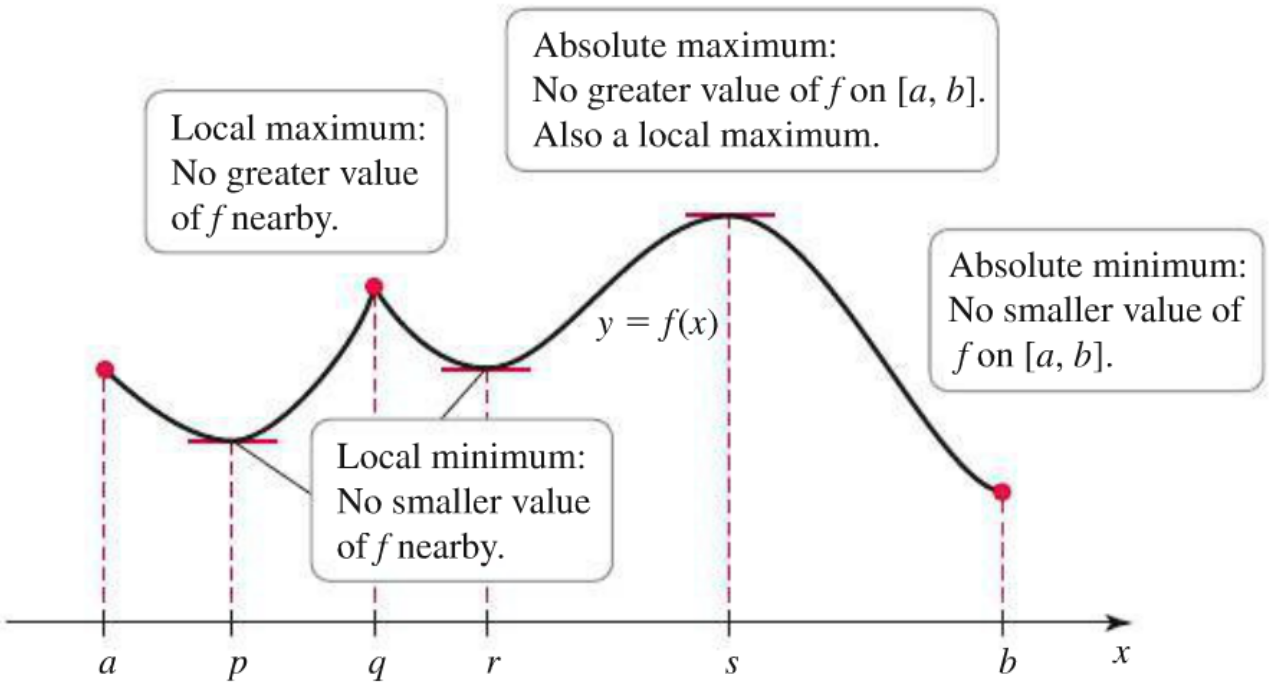
\includegraphics[width=0.55\linewidth]{images/briggs_04_01/fig4_5.png}
\end{center}

\textit{Note:} Local extrema \textbf{CANNOT} occur at endpoints. 

\vspace*{\stretch{1}}
\begin{ex*}
  State the absolute extrema and the local extrema:
\end{ex*}
\begin{center}
  \begin{tikzpicture}
    \begin{groupplot}[
      group style={group size=3 by 2, horizontal sep=1.5cm, vertical sep=1.5cm},
      axis lines=center,
      width=0.325\linewidth,
      axis line style={->},
      ticklabel style={font=\normalsize,inner sep=0.5pt,fill=white,opacity=1.0, text opacity=1},
      xlabel=$x$, xlabel style={at={(ticklabel* cs:1)},anchor=north west},
      ylabel=$y$, ylabel style={at={(ticklabel* cs:1)},anchor=south west},
      every axis plot/.append style={line width=0.95pt, color=blue}
      ]
      \nextgroupplot[
        xmin=1.75, xmax=6,
        ymin=0, ymax=6,
        xtick={2.384,3.506,4.704,5.75},
        xticklabels={$a$, $c_1$, $c_2$, $b$},
        ymajorticks=false,
        ]
        \addplot[-] expression[domain=2.384:5.75, samples=100]{(x-2)*(x-3)*(x-4)*(x-5.125)+2};
        \addplot[soldot] coordinates{(2.384,0.9522)(5.45,6)};
      \nextgroupplot[
        xmin=1.75, xmax=6,
        ymin=0, ymax=3,
        xtick={2.5,4,5.5},
        xticklabels={$a$, $c_1$, $b$},
        ymajorticks=false,
        ]
        \addplot[-] expression[domain=2.5:4,samples=501]{-(4-x)/abs(4-x)*abs(4-x)^(1/3)+2};
        \addplot[-] expression[domain=4:5.5,samples=501]{(4-x)/abs(4-x)*abs(4-x)^(1/3)+2};
        \addplot[holdot] coordinates{(2.5,0.85)(5.5,0.85)};
      \nextgroupplot[
        xmin=-3.5, xmax=2.5,
        ymin=-1.5, ymax=2.5,
        ]
        \addplot[-] expression[domain=-3:0]{-x/3-1};
        \addplot[-] expression[domain=0:1]{3*x-1};
        \addplot[-] expression[domain=1:2]{-2*x+4};
        \addplot[soldot] coordinates{(-3,0)(0,-1)(1,2)(2,0)};
    \end{groupplot}
  \end{tikzpicture}
\end{center}
\vspace*{\stretch{1}}
\pagebreak

\begin{ex*}
  Sketch the graph of a continuous function $f$ on $\sbrkt{0,4}$ satisfying the given properties:
\end{ex*}

\begin{enumerate}
  \item 
    $f'(x)=0$ for $x=1,2$ and $3$; $f$ has an absolute minimum at $x=1$; $f$ has no local extremum at $x=2$; and $f$ has an absolute maximum at $x=3$.

    \begin{tikzpicture}
      \begin{axis}[
        axis lines=center,
        axis line style={->},
        xmin=-0.5, xmax=4.5,
        ymin=-6, ymax=6,
        xtick={-6,-5,...,6},
        height=2.24in,
        width=\linewidth,
        ymajorticks=false,
        ticklabel style={font=\small,inner sep=0.5pt,fill=white,opacity=1.0, text opacity=1},
        ]
      \end{axis}
    \end{tikzpicture}
  \item 
    $f'(1)$ and $f'(3)$ are undefined; $f'(2)=0$; $f$ has a local maximum at $x=1$; $f$ has a local minimum at $x=2$; $f$ has an absolute maximum at $x=3$; and $f$ has an absolute minimum at $x=4$.

    \begin{tikzpicture}
      \begin{axis}[
        axis lines=center,
        axis line style={->},
        xmin=-0.5, xmax=4.5,
        ymin=-6, ymax=6,
        xtick={-6,-5,...,6},
        height=2.24in,
        width=\linewidth,
        ymajorticks=false,
        ticklabel style={font=\small,inner sep=0.5pt,fill=white,opacity=1.0, text opacity=1},
        ]
      \end{axis}
    \end{tikzpicture}
  \item 
    $f'(x)=0$ at $x=1$ and $3$; $f'(2)$ is undefined; $f$ has an absolute maximum at $x=2$; $f$ has neither a local maximum nor a local minimum at $x=1$; and $f$ has an absolute minimum at $x=3$.

    \begin{tikzpicture}
      \begin{axis}[
        axis lines=center,
        axis line style={->},
        xmin=-0.5, xmax=4.5,
        ymin=-6, ymax=6,
        xtick={-6,-5,...,6},
        height=2.24in,
        width=\linewidth,
        ymajorticks=false,
        ticklabel style={font=\small,inner sep=0.5pt,fill=white,opacity=1.0, text opacity=1},
        ]
      \end{axis}
    \end{tikzpicture}
\end{enumerate}
%\vspace*{\stretch{1}}
\pagebreak

\noindent
\fbox{\parbox{0.9875\linewidth}{\textbf{Theorem 4.2: Local Extreme Value Theorem}
  
  If $f$ has a local maximum or minimum value at $c$ and $f'(c)$ exists, then $f'(c)=0$.
}}
\begin{center}
  \textit{Note:} If the derivative is zero, then the function \textbf{MIGHT} have a max/min.  
\end{center}

\begin{ex*}
  Sketch a graph of a function $f(x)$ that has a local maximum value at a point $c$ where $f'(c)$ is defined.
\end{ex*}
\vspace*{\stretch{1}}
\begin{ex*}
  Sketch a graph of a function $f(x)$ that has a local maximum value at a point $c$ where $f'(c)$ is undefined.
\end{ex*}
\vspace*{\stretch{1}}
\begin{ex*}
  Graph 
  \begin{tasks}(2)
    \task $f(x)=x^3$
    \task $f(x)=\abs{x}$
  \end{tasks}
\end{ex*}
\vspace*{\stretch{1}}
\pagebreak
\begin{defn*}[Critical Point]
  An interior point $c$ of the domain of $f$ at which $f'(c)=0$ \textit{or} $f'(c)$ fails to exist is called a \textbf{critical point} of $f$.
\end{defn*}
\begin{ex*}
  Find the critical points of
\end{ex*}
\begin{tasks}[after-item-skip=\stretch{1}, label=~](1)
  \task $f(x)=x^3+3x^2-24x$
  \task $g(x)=\sqrt{4-x^2}$
  \task $h(t)=3t-\sin\inv(t)$
\end{tasks}
\vspace*{\stretch{1}}
\pagebreak
\begin{ex*}
  Find the critical points of
\end{ex*}
\begin{tasks}[after-item-skip=\stretch{1}, label=~](1)
  \task $f(x)=\sin(x)\cos(x)$ on $\sbrkt{0,2\pi}$. 
  \task $f(t)=t^2-2\ln(t^2+1)$
  \task $f(x)=x\sqrt{x-a}$
  \task $f(x)=\sin\inv(x)\cos\inv(x)$
\end{tasks}
\vspace*{\stretch{1}}
\pagebreak
\begin{center}
  \fbox{\parbox{0.8\linewidth}{
    How to find the absolute max/min of $f(x)$ on $\sbrkt{a,b}$:
    \begin{enumerate}
      \item 
        Find $f'(x)$
      \item 
        Find all critical points ($f'(x)=0$ or $f'(x)$ \textbf{DNE})
      \item 
        Evaluate $f(x)$ at the critical points within $\sbrkt{a,b}$ and the end points.
      \item 
        Identify the absolute max and absolute min using the values found. Include value and location (e.g. ordered pair $(x,y)$)
    \end{enumerate}
    }}
\end{center}
\begin{ex*}
  Find the absolute max and min of $f(x)=2x-2x^\frac{2}{3}$ on $\sbrkt{-1,3}$.
\end{ex*}
\vspace*{\stretch{1}}

\begin{ex*}
  Find the absolute max and min of $f(x)=\frac{x}{x^2+1}$ on $\sbrkt{0,2}$.
\end{ex*}
\vspace*{\stretch{1}}

\begin{ex*}
  Find the absolute max and min of $f(x)=3x^4-4x^3-12x^2+1$ on $\sbrkt{-2,3}$.
\end{ex*}
\vspace*{\stretch{1}}
\pagebreak

\begin{ex*}
  Find the absolute max and min of $f(x)=\sin(3x)$ on $\sbrkt{-\frac{\pi}{4},\frac{\pi}{3}}$.
\end{ex*}
\vspace*{\stretch{1}}

\begin{ex*}
  Find the absolute max and min of $f(x)=xe^{1-\frac{x}{2}}$ on $\sbrkt{0,5}$.
\end{ex*}
\vspace*{\stretch{1}}

\begin{ex*}
  Find the absolute max and min of $f(x)=e^x-2x$ on $\sbrkt{0,2}$.
\end{ex*}
\vspace*{\stretch{1}}
\pagebreak

\begin{ex*}
  Find the absolute max and min of $f(x)=x^\frac{1}{3}(x+4)$ on $\sbrkt{-27,27}$.
\end{ex*}
\vspace*{\stretch{1}}

\begin{ex*}
  Find the absolute max and min of $y=\sqrt{x^2-1}$.
\end{ex*}
\vspace*{\stretch{1}}

\begin{ex*}
  Find the absolute/local max and min of $f(x)=x^2\parens{x^2+4x-8}$ on $\sbrkt{-5,2}$.
\end{ex*}
\vspace*{\stretch{1}}
\pagebreak

\begin{ex*}
  \textbf{Minimum-surface-area box} 
  %TODO Future Peter
  % S(x)=2x^2+\frac{4V}{x}
  
  All boxes with a square base of length $x$ and a volume $V$ have a surface area given by $S(x)=x^2+\frac{4V}{x}$. Find $x$ such that the box has volume $50\,ft^3$ with minimal surface area.
\end{ex*}
\vspace*{\stretch{1}}

\begin{ex*}
  \textbf{Trajectory high point}
  
  A stone is launched vertically upward from a cliff $192\,ft$ above the ground at a speed of $64\,ft/s$. Its height above the ground $t$ seconds after the launch is given by $s=-16t^2+64t+192,$ for $0\leq t\leq 6$. When does the stone reach its maximum height?
\end{ex*}
\vspace*{\stretch{1}}
\pagebreak

\begin{ex*}
  \textbf{Maximizing Revenue}
  
  A sales analyst determines that the revenue from sales of fruit smoothies is given by $R(x)=-60x^2+300x$, where $x$ is the price in dollars charged per item, for $0\leq x\leq 5$.
  \begin{enumerate}[label=\alph*)]
    \item 
      Find the critical points of the revenue function.
    \item 
      Determine the absolute maximum value of the revenue function and the price that maximizes the revenue.
  \end{enumerate}
\end{ex*}
\pagebreak

\begin{ex*}
  Find the absolute and local extreme values of the following
  \begin{enumerate}[itemsep=\stretch{1}]
    \item $f(x)=\abs{x-3}+\abs{x+2}$ on $\sbrkt{-4,4}$,
    \item $g(x)=\abs{x-3}-2\abs{x+1}$ on $\sbrkt{-2,3}$.
  \end{enumerate}
\end{ex*}
\vspace*{\stretch{1}}
\pagebreak

\begin{ex*}
  \textbf{Every second counts} (4.01: Q87)
  
  You must get from a point $P$ on the straight shore of a lake to a stranded swimmer who is $50\,m$ from a point $Q$ on the shore that is $50\,m$ from you. Assuming that you can swim at a speed of $2\,m/s$ and run at a speed of $4\,m/s$, the goal of this exercise is to determine the point along the shore, $x$ meters from $Q$, where should you stop running and start swimming to reach the swimmer in the minimum time.

\noindent
\begin{minipage}{0.675\linewidth}
  \begin{enumerate}[label=\alph*)]
    \item 
      Find the function $T$ that gives the travel time as a function of $x$, where $0\leq x\leq 50$.
    \item 
      Find the critical point of $T$ on $(0,50)$.
    \item 
      Evaluate $T$ at the critical point and the endpoints ($x=0$ and $x=50$) to verify that the critical point corresponds to an absolute minimum. What is the minimum travel time?
    \item 
      Graph the function $T$ to check your work.
  \end{enumerate}
\end{minipage}%
\begin{minipage}{0.325\linewidth}
  \begin{flushright}
    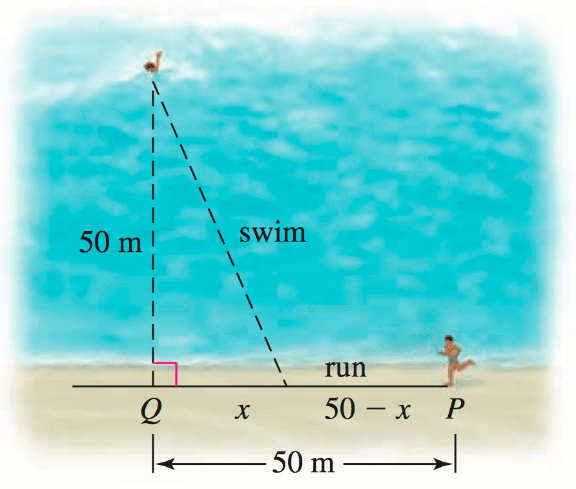
\includegraphics[width=0.95\linewidth]{images/briggs_04_01/swimming_q87.png}
  \end{flushright}
\end{minipage}~
\end{ex*}
\pagebreak

\end{document}
